\chapter{Modified Treatment Policy}
\label{ch-modi-treat}

This chapter is based
primarily on Ref. \cite{han-rot-2013}.
Refs.
\cite{hernan-book}
and \cite{khstats-mtp}
were also very helpful.


A {\bf Modified Treatment Policy (MTP)}
is a generalization
of the Potential
Outcomes (PO)\footnote{PO theory
is discussed in Chapter
 \ref{ch-pot-out}.} model
so as to
modify the original treatment.
This is accomplished
by adding a modified treatment
dose node $\ul{\tilx}$
acting as a mediator
between the treatment dose node 
$\rvx$ and the treatment effect node $\rvy$ (i.e., by considering
$\rvx\rarrow\ul{\tilx}\rarrow \rvy$).

\section{One time MTP}
Consider a typical PO bnet $G$
and its corresponding imagined bnet $G_{im2}$ (see Fig.\ref{fig-modi-po})\footnote{ Ref.\cite{han-rot-2013} uses the
notation $L = \rvc$,
$A = \rvx$, $Y=\rvy$,
$Y_q=\rvy(\tilx)$,
 $Q=\ul{\tilx}$. Furthermore, it does not 
display a DAG.
}.
A MTP adds a Bayesian prior to the
 node $\ul{\tilx}$ in $G_{im2}$.
The prior depends on the treatment
dose variable (a.k.a. exposure variable) $\rvx$ and its parents $pa(\rvx)=\rvc$.
This adds 
to $G_{im2}$  new arrows $\rvc\rarrow\ul{\tilx}$
and $\rvx\rarrow \ul{\tilx}$ (see Fig.\ref{fig-unmodi-modi}).


\begin{figure}[h!]
$$
\begin{array}{ccc}
\xymatrix{
\rvc
\ar[dd]\ar[ddrr]
\\
\\
\rvx \ar[rr]
&
&\rvy
}
&
\xymatrix{
\rvc
\ar[dd]\ar[dr] \ar[drr]
\\
& \rvy(0)\ar[dr]
&\rvy(1)\ar[d]
\\
\rvx\ar[rr]
&
&\rvy
}
&
\xymatrix{
\rvc
\ar[dd]\ar[dr] \ar[drr]
\\
& \rvy(0)\ar[dr]
&\rvy(1)\ar[d]
\\
\rvx
&\ul{\tilx}=\tilx\ar[r]
&\rvy
}
\\
G
&G_{im1} =\cali_{\rvx\rarrow\rvy} G
& G_{im2}=\cali_{\ul{\tilx}\rarrow\rvy}\cali_{\rvx\rarrow\rvy}(\tilx)G
\end{array}
$$
\caption{$G$ is one of the
simplest possible bnets considered in  PO theory.
In the usual PO theory,
one only considers the bnet $G_{im1}$.
In MTP theory, we
consider the bnet $G_{im2}$.
For $G_{im2}$, $\tilx\in S_{\ul{\tilx}}= 
S_\rvx=\bool$.} (
As usual in this book, $S_\rva$
denotes the set of
values that a random variable
$\rva$ can assume.
Imagine operators such as
$\cali_{\rvx\rarrow \rvy}$
and $\cali_{\rvx\rarrow \rvy}(\tilx)$ 
are discussed in Chapter \ref{ch-counterf}.
)
\label{fig-modi-po}
\end{figure}


\begin{figure}[h!]
$$
\begin{array}{cc}
\xymatrix{
pa(\rvx) =\rvc
\ar[dd]
&
&pa'(\rvy)\ar[d]
\\
&&[\rvy(\tilx)]_{\tilx\in S_{\ul{\tilx}}}\ar[d]
\\
\rvx
&\ul{\tilx}=\tilx\ar[r]
&\rvy
}
&
\xymatrix{
pa(\rvx)=\rvc
\ar[dd]\ar[ddr]
&
&pa'(\rvy)\ar[d]
\\
&&[\rvy(\tilx)]_{\tilx\in S_{\ul{\tilx}}}\ar[d]
\\
\rvx\ar[r]
&\ul{\tilx}\ar[r]
&\rvy
}
\\
G_{im2}
 &G_{im2,mod}
\end{array}
$$
\caption{In this figure, $G_{im2}$
is the generalization of the $G_{im2}$
in Fig.\ref{fig-modi-po}.
Note that $pa'(\rvy)$ are the parents in $G$ of
$\rvy$, excluding $\rvx$.
Note that $S_{\ul{\tilx}}\subset S_\rvx$. }
\label{fig-unmodi-modi}
\end{figure}

The TPM, printed in  blue, for node $\ul{\tilx}$
of the imagined bnet $G_{im2}$ in Fig.\ref{fig-unmodi-modi}, is as follows
\beq\color{blue}
P(\ul{\tilx}=\tilx; x) =\delta(\tilx, x)
\eeq

The TPM, printed in  blue, for node $\ul{\tilx}$
of the modified imagined bnet $G_{im2,mod}$ in Fig.\ref{fig-unmodi-modi},
 is as follows
\beq\color{blue}
P(\ul{\tilx}=\tilx | \rvx=x, c)= \text{ prior}
\eeq

Hence, node $\ul{\tilx}$
has a non-informative (frequentist) prior in $G_{im2}$,
and it has an informative (Bayesian) prior in $G_{im2,mod}$.

The following
assumptions will
be made about $G_{im2, mod}$:

\begin{enumerate}


\item {\bf Consistency (a.k.a. SUTVA)}

The TPM, printed in  blue, for node $\rvy$
of the modified imagined bnet $G_{im2,mod}$ in Fig.\ref{fig-unmodi-modi},
 is as follows

\beq \color{blue}
P(y\cond \tilx, \{y(\tilx')\}_{\tilx'\in S_{\ul{\tilx}}})=
\indi(
\quad y =\sum_{\tilx'\in S_{\ul{\tilx}}}
 y(\tilx')\indi(\tilx'=\tilx)
 \quad)
\eeq
When $S_{\ul{\tilx}}=\bool$,
this becomes the more familiar 
statement from standard 
PO theory:

\beq \color{blue}
P(y\cond \tilx, \{y(0), y(1)\})=
\indi(\quad y =
y(0)(1-\tilx)
+ 
y(1)\tilx
\quad)
\eeq

An immediate consequence
of this deterministic TPM for
node $\rvy$ is that
\beqa
P(\rvy=y|\tilx, pa'(\rvy)=\xi)&=&
P(\rvy(\tilx)=y|\tilx, pa'(\rvy)=\xi)
\eeqa


\item {\bf Exchangeability (a.k.a.
conditional independence assumption (CIA))}

\beqa
P(\rvy(\tilx')=y|\tilx, pa'(\rvy)=\xi)
&=&
P(\rvy(\tilx')=y|pa'(\rvy)=\xi)
\eeqa

CIA follows from the structure
of the DAG $G_{im2,mod}$,
because in that
DAG, fixing the value
of $pa'(\rvy)$
blocks messages from $\ul{\tilx}$
to $\rvy(\tilx)$ (i.e.,
for all $\tilx\in S_{\ul{\tilx}}$,
we have  
$\ul{\tilx}
\perp \rvy(\tilx)|pa'(\rvy)$.)

\item {\bf Identifiability}

We must have
\beq
S_{\ul{\tilx}} \subset S_\rvx
\eeq
in $G_{im2, mod}$
or else queries of the type
 $P(\rvy(\tilx)=y|pa'(\rvy)=\xi)$ are not identifiable.
This is clear because if $\tilx\not\in S_\rvx$,
then we have no information of the type

\beq
P(\rvy=y|\tilx, pa'(\rvy)=\xi)=P(\rvy(\tilx)=y|pa'(\rvy)=\xi
)\;.
\eeq

\item{\bf Positivity}

Define the following 2 propensities
for $x\in S_\rvx$ and $\tilx \in S_{\ul{\tilx}}$:

\beq
g_{x|c}=P(\rvx=x |c)
\eeq

\beq
\tilg_{\tilx|c}=P(\ul{\tilx}=\tilx |c)
\eeq

Positivity for  $G_{im2,mod}$
is the requirement that

\beq
0<g_{\tilx|c}<1 \text{ for all $\tilx \in S_{\ul{\tilx}}$ and $c\in S_\rvc$}
\eeq
If $g_{\tilx|c}$
is deterministic, then this requirement
is not satisfied, and we cannot do IPW (i.e.,
inverse propensity weighing).

Note that using a MDP can allow IPW to
be performed  in cases
when the propensity $g_{x|c}$
is anomalous
(i.e., is
either not defined
or violates positivity)
for some $x\in S_\rvx$, but is not anomalous
for all $\tilx\in S_{\ul{\tilx}}$, where
$S_{\ul{\tilx}}$
is some proper subset of $S_\rvx$.

\end{enumerate}

The probability
distribution
$P(\tilx|x, c)$ (i.e., the  $\ul{\tilx}$ prior for $G_{im2,mod}$)
is called the MTP.
An MTP can be either
deterministic or probabilistic.
An MTP that depends (resp., does not depend)
 on $x$ is said to
be dynamic (resp., static), because $\tilx$ depends (resp., does not
depend) on the previous value
of $x$.

\begin{enumerate}
\item Deterministic MTP

Suppose $S_{\ul{\tilx}}\subset S_\rvx$
and we are given a function
$\tilx_c(\cdot):S_\rvx\rarrow S_{\ul{\tilx}}$.
Then let the TPM, printed
in blue, for node $\ul{\tilx}$, be as follows:

\beq\color{blue}
P(\ul{\tilx}=\tilx | \rvx=x, c)= \delta(\tilx, \tilx_c(x))
\eeq

\begin{figure}[h!]
\centering
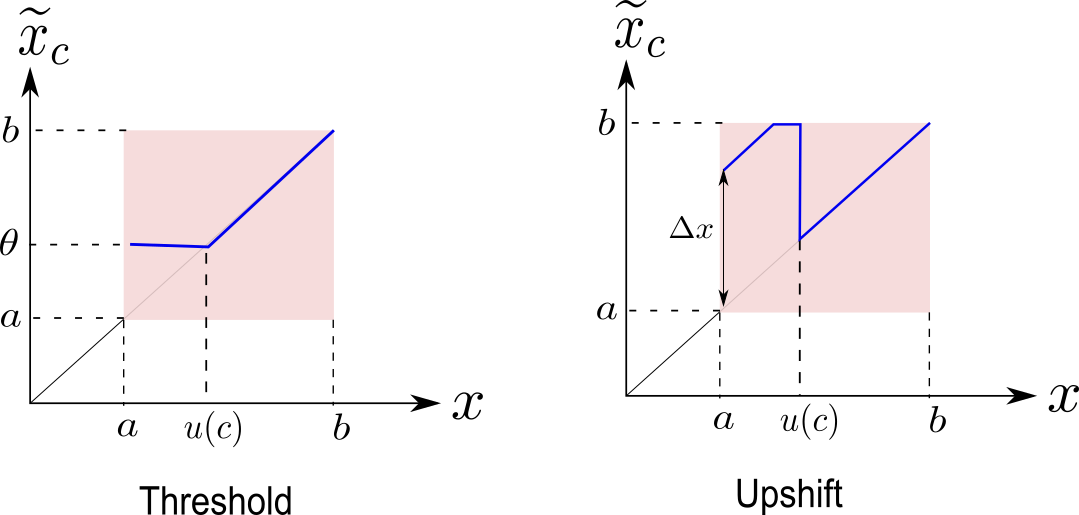
\includegraphics[width=4in]
{modi-treat/det-mtps.png}
\caption{Two possible  
maps $\tilx_c:[a,b]\rarrow [a,b]$
for a deterministic MTP. }
\label{fig-det-mtps}
\end{figure}

Examples of $\tilx_c(x)$: 
\begin{itemize}

\item threshold in
the value of $x$ for small 
values of $x$. (See Fig.\ref{fig-det-mtps})

Let $S_\rvx=[a,b]$ where $a<b$.
For some $\theta\in[a, b]$ and $u(c)\in [a,b]$,
set

\beq
\tilx_c(x) = \left\{\begin{array}{ll}
\theta &\text{ if }x\leq u(c)
\\
x &\text{ if }x> u(c)
\end{array}
\right.
\eeq

\item upshift in
the value of $x$ for small 
values of $x$. (See Fig.\ref{fig-det-mtps})

Let $S_\rvx=[a,b]$ where $a<b$.
For some $\Delta x >0$,
and $u(c)\in[a,b]$, set

\beq
\tilx_c(x) = \left\{\begin{array}{ll}
(x +  \Delta x) &\text{ if }x< u(c)\text{ and }
(x +  \Delta x)\in[a,b]
\\
x &\text{ if }x> u(c)
\\
b & \text{ if }(x +  \Delta x)>b
\end{array}
\right.
\eeq



\end{itemize}


\item Stochastic MTP

For some
convenient, user specified,
probability
distribution
$P(\tilx| x', x, c)$,
where $\tilx\in S_{\ul{\tilx}}$,
$x,x'\in S_\rvx$,
 and $c\in S_\rvc$,
let the TPM, printed
in blue, for node $\ul{\tilx}$, be as follows:


\beq\color{blue}
P(\tilx|x,c)=
\sum_{x'\in S_\rvx} P(\tilx| x', x, c)
\underbrace{P(\rvx=x'|c)}_{\text{unmodified propensity}}
\eeq

Examples
\begin{itemize}
\item
Suppose we are given a function $x_c:S_{\ul{\tilx}}\rarrow S_\rvx$.
($x_c(\tilx)$ could be the inverse, if
 it exists, of the function $\tilx_c(x)$
defined in the deterministic TMP case.)

\beq
P(\tilx|x,c) = \frac{P(\rvx=x_c(\tilx)|c)}{\sum_\tilx numerator}
\eeq

\item
Suppose
$S_\rvx=S_{\ul{\tilx}}=\bool$, $\theta\in\RR$,
and let


\beq
P(\tilx|x, c)
=
[\pi(x,c)]^{\tilx} [1-\pi(x,c)]^{1-\tilx}
\eeq
where

\beq
\pi(x,c)=
\frac{\theta^x P(\rvx=x|c)}{\sum_x numerator}
\eeq

\end{itemize}


\end{enumerate}



\section{$\Delta_{|c}$ estimand}

Let
\beqa
\caly_{|x, c}
&=&
\sum_y y P(\rvy(x)=y\cond x, c)
\\
&=& \sum_y y P(\rvy=y\cond x, c)
\eeqa

\beqa
\TIL{\caly}_{|\ul{\tilx}=\tilx, c}
&=&
\sum_y y P(\rvy(\tilx)=y\cond \tilx, c)
\\
&=&
\sum_y y P(\rvy=y\cond \tilx, c)
\eeqa

\beqa
\TIL{\caly}_{|\rvx=x, c}
&=&
\sum_\tilx
\TIL{\caly}_{|\ul{\tilx}=\tilx, c}
P(\tilx|x,c)
\eeqa

\beq
\caly_{|c} = \sum_{x} \caly_{|x, c}P(x|c)
,\quad \caly =\sum_c P(c)\caly_{|c}
\eeq

 
\beq
\TIL{\caly}_{|c} = \sum_{x} \TIL{\caly}_{|\rvx=x, c}P(x|c)
,\quad \TIL{\caly} =\sum_c P(c)\TIL{\caly}_{|c}
\eeq

Note that there
are two $\TIL{\caly}$,
namely
 $\TIL{\caly}_{|\rvx=x,c}$
 and
 $\TIL{\caly}_{|\ul{\tilx}=\tilx,c}$.

Define the $\Delta_{|c}$ estimand by:

\beq
\Delta_{|c} = \caly_{|c} -\TIL{\caly}_{|c},\quad \Delta = \sum_c P(c)\Delta_{|c}
\eeq
$\Delta_{|c}$  measures the 
difference between the real world 
represented by $\caly_{|c}$
and a modified world
represented by $\TIL{\caly} _{|c}$.

\begin{claim}
Consider the deterministic MTP case $P(\tilx|x,c)=
\delta(\tilx , \tilx_c(x))$,
where the function $\tilx=\tilx_c(x)$ is
invertible with inverse $x=x_c(\tilx)$
for some $x\in \XX\subset \RR$.
Then, 

\beq
\TIL{\caly}_{|\rvx=x, c}=
\caly_{|x_c(\tilx), c}
\eeq
\end{claim}
\proof


\beqa
\TIL{\caly}_{|\rvx=x, c} &=&
\sum_\tilx\sum_y y P(\rvy=y\cond \ul{\tilx}=\tilx, c)
\delta(\tilx, \tilx_c(x))
\\
&=&
\sum_y y P(\rvy=y\cond \ul{\tilx}=\tilx_c(x), c)
\\
&=&
\sum_y y P(\rvy=y\cond \rvx=x_c(\tilx), c)
\\
&=&
\caly_{|x_c(\tilx), c}
\eeqa
\qed



Henceforth
in this chapter, we will
restrict  our attention to the
deterministic MTP case in which
$P(\tilx|x,c)=\delta(\tilx, \tilx_c(x))$.
We will also
assume that
the domain of $\tilx_c(x)$
is a union of disjoint sets $\XX^j_c$
for $j=1,2, \dots, nj(c)$,
and that on each set $\XX^j_c$,
$\tilx_c(x)$ is invertible and differentiable.

\beq
\left\{
\begin{array}{l}
\XX= S_\rvx
\\
\XX_{c}^j \cap \XX_{c}^{j'}=
\emptyset \text{ for } j\neq j'
\\
\XX_c = \cup_{j=1}^{nj(c)}
\XX_{c}^j\subset \XX
\end{array}
\right.
\eeq

\beq
\tilx_c(x) =\sum_{j=1}^{nj(c)}  \indi(x\in \XX_c^j)\tilx_c^j(x)
\eeq


\beq
P(\tilx|x, c)=\delta(\tilx, \tilx_c(x))=
\sum_j \indi(x\in \XX_c^j)
\delta(\tilx, \tilx^j_c(x))
\eeq

\beq
(\tilx^j_c)^{-1}(\tilx)= x^j(\tilx)
\eeq

\beq
\TIL{\XX}_c^j= \tilx^j_c(\XX^j_c)=\{\tilx^j_c(x): x\in \XX^j_c\}
\eeq

\beq
P_{\XX_c} = P(\rvx\in \XX_c)
\eeq

\begin{claim}

\beq
\TIL{\caly}_{|c}=
\frac{1}{P_{\XX_c}}
E_{\ul{\tilx}|c}[
\lam_c(\tilx)\caly_{|x_c(\tilx),c}]
\;,
\label{eq-til-caly-c}
\eeq

\beqa
\caly_{|c}&=&
\frac{1}{P_{\XX_c}}
E_{\ul{\tilx}|c}[
\lam_c(\tilx)\caly_{|\tilx, c}]
\label{eq-caly-c}
\eeqa
and

\beq
P_{\XX_c} =
E_{\ul{\tilx}|c}[
\lam_c(\tilx)]
\label{eq-prob-xx}
\eeq
where\footnote{$\lam_c(\tilx)$
is just a piecewise Jacobian.
In Ref.\cite{han-rot-2013},
the part of Eq.(\ref{eq-lam-c-tilx})
which is marked as being equal to 1
is incorrectly assumed to be different from 1.
}

\beq
\lam_c(\tilx)=
\sum_j \indi(\tilx\in \TIL{\XX}^j_c)
\der{x^j_c(\tilx)}{\tilx}
\underbrace{\frac{P(\rvx=x^j_c(\tilx)|c)}{P(\ul{\tilx}=\tilx|c)}
}_{=1}
\label{eq-lam-c-tilx}
\eeq
\end{claim}
\proof

\begin{align}
\TIL{\caly}_{|c}
&=
\frac{1}{P_{\XX_c}}
\int_{x\in \XX_c}dx\;P(x|c)
\sum_y y P(y|\ul{\tilx}=\tilx_c(x), c)
\\
&=
\frac{1}{P_{\XX_c}}
\sum_j \int_{x\in\XX^j_c} dx\;P(x|c)
\sum_y y P(y|\ul{\tilx}=\tilx_c^j(x),c)
\\
&=
\frac{1}{P_{\XX_c}}
\sum_j
\int_{\tilx\in \TIL{\XX}^j_c}
 d\tilx\; P(\tilx|c)
\der{x^j_c(\tilx)}{\tilx}
\frac{P(\rvx=x^j_c(\tilx)|c)}{P(\tilx|c)}
\underbrace{\sum_y y P(y|\rvx=x_c^j(\tilx),c)}_{\caly_{|x_c^j(\tilx),c}}
\\
&=
\frac{1}{P_{\XX_c}}\int_{\tilx\in \TIL{\XX}_c}
 d\tilx\; P(\tilx|c)
\lam_c(\tilx)
\caly_{|x_c(\tilx),c}
\quad\text{(see Eq(\ref{eq-lam-c-tilx}))}
\\
&=
\frac{1}{P_{\XX_c}}
E_{\ul{\tilx}|c}[
\lam_c(\tilx)\caly_{|x_c(\tilx),c}]
\end{align}

To get  Eq.(\ref{eq-caly-c}), 
replace $\caly_{|x_c(\tilx), c}$ by 
$\caly_{\tilx, c}$
in Eq.(\ref{eq-til-caly-c}).

To get  Eq.(\ref{eq-prob-xx}), 
replace $\caly_{|x_c(\tilx), c}$ by 1
in Eq.(\ref{eq-til-caly-c}).
\qed

From the last claim, it follows that
\beq
\Delta_{|c} = \frac{E_{\rvy, \ul{\tilx}|c}\left[
\lam_c(\tilx)
(y-\caly_{|x_c(\tilx),c})\right]}
{E_{\ul{\tilx}|c}[
\lam_c(\tilx)]}
\eeq


\section{Estimates of $\Delta_{|c}$}

\subsection{Empirical estimate of $\Delta_{|c}$ }
Consider a population $\Sigma$
of individuals $\s\in \Sigma$,
with $|\Sigma|=N$.

Let
\beq
N_c =\sum_\s \delta(c_\s, c)
\;,
\eeq

\beq
P(\s|c)= \frac{\delta(c_\s, c)}{N_c}
\;,
\eeq
and

\beq
E_{\s|c}[\xi_\s] =\sum_\s P(\s|c) \xi_\s
\;.
\eeq
Then set

\beq
\HAT{\Delta}_{|c} = \frac{E_{\s|c}\left[
\lam_{c}(\tilx_\s)
(y_\s-\caly_{|x_{c}(\tilx_\s),c})\right]}
{E_{\s|c}[
\lam_c(\tilx_\s)]}
\eeq

\subsection{OR estimate of $\Delta_{|c}$}

{\bf Outcome Regression (OR)} estimate
of $\Delta_{|c}$.

Calculate the
following estimates in this order:
$\HAT{\tau}
\rarrow\HAT{\Delta}_{|c}$.

Steps:
\begin{enumerate}
\item Calculate $\HAT{\tau}$

Let
\beq
{X}^T= [1, \tilx, c],\quad {X}_\s^T= [1, \tilx_\s, c_\s]
\;.
\eeq
Use Generalized 
Linear Modeling (GLM)\footnote{GLM
is discussed in Chapter \ref{ch-gen-lin-mod}.}
to approximate $y_\s$:

\beq
y_\s \approx \HAT{y}(X_\s^T\HAT{\tau})
\eeq

\beq
\HAT{y}(X_\s^T\HAT{\tau})= g^{-1}(X_\s^T\HAT{\tau})
\eeq
where $g()$ is the link function.

\item Calculate $\HAT{\Delta}_{|c}$

\beq
\HAT{\Delta}_{|c}=\frac{E_{\s|c}[
\lam_c(\tilx_\s) (y_\s - \HAT{y}(X_\s^T\HAT{\tau}))]}
{E_{\s|c}[
\lam_c(\tilx_\s)]}
\label{eq-or-est}
\eeq

\end{enumerate}


 	






\begin{claim} (Asymptotic behavior
of OR estimate)

As $N\rarrow \infty$,

\beq
\sqrt{N_c}(\HAT{\Delta}_{|c}-\Delta^*_{|c})
\rarrow \caln(0, \calv)
\eeq
where

\beq
\calv =
E_{\s|c}[
(IF_\s)^2]
\eeq

\beq
IF_\s = \frac{ R_\s(\HAT{\tau}, \HAT{\Delta}_{|c}) + B(\HAT{\tau})}{C}
\eeq

\beq
R_\s(\tau, \Delta_{|c}) =
\lam_c(\tilx_\s)(y_\s - \HAT{y}(X_\s^T\tau)
-\Delta_{|c})
\eeq

\beq
C=-E_{\s|c}[
\lam_c(\tilx_\s)]
\eeq

\beq
B(\tau) =
\sum_i E_{\s|c}\left[
\lam_c(\tilx_\s)\pder{\HAT{y}(X^T_\s\tau)}{\tau_i}\right]
\frac{E_{\s|c}[S_{i,\s}(\tau)]}
{E_{\s|c}\left[\pder{S_{i,\s}(\tau)}{\tau_i}\right]}
\eeq
(Note that index $i$
labels the components of 
the  column vector $\tau$)
\end{claim}
\proof

Eq.(\ref{eq-or-est}) that defines the OR estimate
can be rewritten as
\beq
0=E_{\s|c}[ \underbrace{
\lam_c(\tilx_\s)(y_\s - \HAT{y}(X_\s^T\HAT{\tau})
-\HAT{\Delta}_{|c})}_{R_\s(\HAT{\tau}, \HAT{\Delta}_{|c})}]
\eeq
If we Taylor
expand $R_\s(\HAT{\tau}, \HAT{\Delta}_{|c})$
to first order in each of its 2
estimator arguments, we get


\beq
E_{\s|c}[R_\s(\HAT{\tau}, \HAT{\Delta}_{|c}) ]=
\left\{
\begin{array}{l}
\underbrace{E_{\s|c}[R_\s(\tau^*, \Delta^*_{|c})
]}_{A}
\\
+\sum_i
\underbrace{E_{\s|c}\left[\pder{R_\s(\tau^*, \Delta^*_{|c})}{\tau^*_i}
\right] }_{B_i}
(\HAT{\tau}_i - \tau^*_i)
\\
+
\underbrace{E_{\s|c}\left[\pder{R_\s(\tau^*, \Delta^*_{|c})} {\Delta^*_{|c}}
 \right] }_{-C}
(\HAT{\Delta}_{|c} - \Delta^*_{|c})
\end{array}
\right.
\eeq
Solving the last equation for
$\HAT{\Delta}_{|c} - \Delta^*_{|c}$ 
yields
\beq
\HAT{\Delta}_{|c} - \Delta^*_{|c}=
\frac{A +
\overbrace{\sum_i B_i(\HAT{\tau}_i - \tau^*_i)}^{B}}
{C}
\eeq

Assuming $y_\s\in \bool$,
define the Cross Entropy
and its first derivative
with respect to $\tau_i$ by
\beq
CE_\s=\sum_{y_\s=0,1} y_\s \ln \HAT{y}(X_\s^T\tau)
\eeq

\beq
S_{i,\s}(\tau)=
\pder{CE_\s}{\tau_i}
\eeq
In this notation,
according to the maximum likelihood principle,
the best choice of parameters $\tau_i$
must satisfy 
\beq
0=E_{\s|c}[S_{i,\s}(\HAT{\tau})]
\eeq
If we Taylor
expand $S_{i,\s}(\HAT{\tau})$
to first order in its
estimator argument, we get

\beq
E_{\s|c}[S_{i,\s}(\HAT{\tau})]= E_{\s|c}[S_{i,\s}(\tau^*)]
+
E_{\s|c}\left[\pder{S_{i,\s}(\tau^*)}{\tau_i}\right]
(\HAT{\tau}_i-\tau_i^*)
\eeq
Hence,

\beq
\HAT{\tau}_i-\tau_i^*=
-\;\frac{E_{\s|c}[S_{i,\s}(\tau^*)]}
{E_{\s|c}\left[\pder{S_{i,\s}(\tau^*)}{\tau_i}\right]}
\;.
\eeq
Now putting our
previous results together, we get

\beqa
A &=&
E_{\s|c}[R_\s(\tau^*, \Delta^*_{|c})]
\\
&=&
E_{\s|c}[
\lam_c(\tilx_\s)(y_\s - \HAT{y}(\xtau^*)
-\Delta^*_{|c})]
\eeqa

\beq
B_i= -E_{\s|c}\left[
\lam_c(\tilx_\s)\pder{\HAT{y}(\xtau^*)}{\tau^*_i}\right]
\eeq

\beqa
B(\tau^*) &=& \sum_i B_i (\HAT{\tau}_i-\tau^*_i)
\\
&=&
\sum_i E_{\s|c}\left[
\lam_c(\tilx_\s)\pder{\HAT{y}(\xtau^*)}{\tau^*_i}\right]
\frac{E_{\s|c}[S_{i,\s}(\tau^*)]}
{E_{\s|c}\left[\pder{S_{i,\s}(\tau^*)}{\tau_i}\right]}
\eeqa


\beq
C=-E_{\s|c}[
\lam_c(\tilx_\s)]
\eeq

\beq
IF_\s = \frac{ R_\s(\HAT{\tau}, \HAT{\Delta}_{|c}) + B(\HAT{\tau})}{C}
\eeq

\beq
\calv =
E_{\s|c}[
(IF_\s)^2]
\eeq
\qed
\subsection{IPW estimate of $\Delta_{|c}$}
{\bf Inverse Propensity Weighted (IPW)}
estimate.
Calculate the
following estimates in this order:
$\HAT{\tau}
\rarrow\HAT{\theta}
\rarrow\HAT{\Delta}_{|c}$


\subsection{DR estimate
of $\Delta_{|c}$}

{\bf Doubly Robust (DR)} estimate.
Calculate the
following estimates in this order:
$\HAT{\tau}
\rarrow\HAT{\theta}
\rarrow\HAT{\gamma}
\rarrow\HAT{\Delta}_{|c}$

\section{Other Estimands besides $\Delta_{|c}$}

Suppose $\tilx_0, \tilx_1\in S_{\ul{\tilx}}$.
Define the
{\bf Modified ATE (MATE)} by

\beq
MATE_{|c} = \TIL{\caly}_{|\ul{\tilx}=\tilx_1, c}
-
\TIL{\caly}_{|\ul{\tilx}=\tilx_0, c}
\eeq

\beq
MATE = \sum_c P(c) MATE_{|c}
\eeq



\section{Multi-time MTP}
A g-formula
is any formula that
defines recursively the full
probability distribution of a bnet.
In other words, it's a recursive
definition of a Dynamical Bayesian Network.\footnote{Dynamical
Bayesian Networks
are discussed in Chapter \ref{ch-dyn-bnet}.}


Let's
define a g-formula\footnote{
Chapter
\ref{ch-g-formula} defines
a different g-formula
that we call a sequential
backdoor g-formula.}
for
Multi-time (a.k.a. longitudinal) MTP (LMTP).

Consider  $t=1,2, \ldots, nt$,

For $nt=1$,

\beq
\begin{array}{cc}
\xymatrix{
\rvc_1\ar[d]\ar[dr]
\\
\rvx_1\ar[r]
&\rvy
}
 &
\xymatrix{
\rvc_1\ar[d]\ar@/^1pc/[dd]\ar[ddr]
\\
\rvx_1\ar[d]
\\
\ul{\tilx}_1\ar[r]
&\rvy
}
\end{array}
\eeq

\beq
P(y,x_1, c_1)=
P(y|x_1, c_1)
P(x_1|c_1)
P(c_1)
\eeq

\beq
P(y,\tilx_1,x_1, c_1)=
P(y|\tilx_1, c_1)
P(x_1|c_1)
P(\tilx_1|x_1, c_1)P(c_1)
\eeq
For $nt=2$,

\beq
\begin{array}{ll}
\xymatrix{
\rvc_1\ar[d]\ar[r]\ar[dr]
&\rvc_2\ar[d]\ar[rd]
\\
\rvx_1\ar[r] \ar[ru]
&\rvx_2\ar[r]
&\rvy
}
&
\xymatrix{
\rvc_1\ar[d]\ar[r]\ar@/^1pc/[dd]\ar[ddr]\ar[dr]
&\rvc_2\ar[d]\ar@/^1pc/[dd]\ar[ddr] \ar[rdd]
\\
\rvx_1\ar[d]
&\rvx_2\ar[d]
\\
\ul{\tilx}_1\ar[ru] \ar[ruu] \ar[r]
&\ul{\tilx}_2\ar[r]
&\rvy
}
\end{array}
\eeq

\beq
P(y,x_{\leq 2},c_{\leq 2})=
\left\{
\begin{array}{l}
P(x_1|c_1) P(c_1)
\\
*P(x_2|x_1, c_{2,1})P(c_2|x_1, c_1)
\\
*P(y|x_2, c_2)
\end{array}
\right.
\eeq

\beq
P(y,\tilx_{\leq 2}, x_{\leq 2},c_{\leq 2})=
\left\{
\begin{array}{l}
P(x_1|c_1)
P(\tilx_1|x_1, c_1) P(c_1)
\\
*P(x_2|\tilx_1, c_{2,1})
P(\tilx_2|x_2, c_{2,1})
P(c_2|\tilx_1, c_1)
\\
*P(y|\tilx_2, c_2)
\end{array}
\right.
\eeq


For $nt=3$,

\beq
\begin{array}{cc}
\xymatrix{
\rvc_1\ar[d]\ar[r]\ar[dr]
&\rvc_2\ar[d]\ar[r]\ar[dr]
&\rvc_3\ar[d] \ar[rd]
\\
\rvx_1\ar[r]\ar[ru]
&\rvx_2\ar[r]\ar[ru]
&\rvx_3\ar[r]
&\rvy
}
&
\xymatrix{
\rvc_1\ar[d]\ar[r]\ar[ddr]\ar[dr]\ar@/^1pc/[dd]
&\rvc_2\ar[d]\ar[r]\ar[ddr] \ar[dr]\ar@/^1pc/[dd]
&\rvc_3\ar[d]\ar[ddr] \ar@/^1pc/[dd] \ar[rdd]
\\
\rvx_1\ar[d]\ar[rd]
&\rvx_2\ar[d]\ar[rd]
&\rvx_3\ar[d]
\\
\ul{\tilx}_1\ar[ru] \ar[ruu] \ar[r]
&\ul{\tilx}_2\ar[ru]\ar[ruu]  \ar[r]
&\ul{\tilx}_3\ar[r]
&\rvy
}
\end{array}
\label{eq-modi-bnet-nt-3}
\eeq

\beq
P(y, x_{\leq 3}, c_{\leq 3})
=
\left\{
\begin{array}{l}
P(x_1|c_1) P(c_1)
\\
*P(x_2|x_1, c_{2,1})P(c_2| x_1, c_1)
\\
*P(x_3|x_{2}, c_{3,2}) P(c_3|x_2, c_2)
\\
*P(y| x_3, c_3)
\end{array}
\right.
\eeq


\beq
P(y,\tilx_{\leq 3}, x_{\leq 3}, c_{\leq 3})
=
\left\{
\begin{array}{l}
P(x_1|c_1)
P(\tilx_1|x_1, c_1)P(c_1)
\\
*P(x_2|\tilx_1, c_{2,1})
P(\tilx_2|\tilx_1, x_{2,1}, c_{2,1})  P(c_2|\tilx_1, c_1)
\\
*P(x_3|\tilx_{2}, c_{3,2})
P(\tilx_3|\tilx_{2}, x_{3,2}, c_{3,2}) P(c_3|\tilx_2, c_2)
\\
*P(y|\tilx_3, c_3)
\end{array}
\right.
\eeq

In general,

\beq
P(y,x_{\leq nt}, c_{\leq nt})=
\left\{
\begin{array}{l}
\prod_{t=1}^{nt}
\{
P(x_t|x_{t-1}, c_{t, t-1} )
P(c_t|x_{t-1}, c_{t-1})
\}
\\
*P(y|x_{nt}, c_{nt})
\end{array}
\right.
\eeq

\beq
P(y,\tilx_{\leq nt},x_{\leq nt}, c_{\leq nt})=
\left\{
\begin{array}{l}
\prod_{t=1}^{nt}
P(x_t|\tilx_{t-1}, c_{t, t-1} )
P(\tilx_t|\tilx_{t-1}, x_{t,t-1}, c_{t, t-1})
P(c_t|\tilx_{t-1},  c_{t-1})
\\
*P(y|\tilx_{nt},x_{nt}, c_{nt})
\end{array}
\right.
\eeq



Note that Ref.\cite{hernan-book} by Hern\'{a}n and Robins  (HR) uses the
notation $L_{t} = \rvc_{t}$,
$A_{t} = \rvx_{t}$
for $t=1, 2, \ldots, nt$. Hence, the $nt=3$ bnet
Eq.(\ref{eq-modi-bnet-nt-3}), written in the HR notation, is
as follows
(before and after adding the $\TIL{A}$ nodes):
\beq
\begin{array}{cc}
\xymatrix{
L_1\ar[d]\ar[r]\ar[dr]
&L_2\ar[d]\ar[r]\ar[dr]
&L_3\ar[d]\ar[rd]
\\
A_1\ar[r]\ar[ru]
&A_2\ar[r]\ar[ru]
&A_3\ar[r]
&\rvy
}
&
\xymatrix{
L_1\ar[d]\ar[r]\ar[ddr]\ar[dr]\ar@/^1pc/[dd]
&L_2\ar[d]\ar[r]\ar[ddr] \ar[dr]\ar@/^1pc/[dd]
&L_3\ar[d]\ar[ddr] \ar@/^1pc/[dd]
\\
A_1\ar[d]\ar[rd]
&A_2\ar[d]\ar[rd]
&A_3\ar[d]
\\
\TIL{A}_1\ar[ru]\ar[r]
&\TIL{A}_2\ar[ru]\ar[r]
&\TIL{A}_3\ar[r]
&\rvy
}
\end{array}
\eeq
HR doesn't actually display the $\TIL{A}$
nodes in its DAGs. Furthermore, in HR,
 nodes $A_t$ and $L_t$
have parent nodes
that are time steps $0,1,2,3,\ldots $ in the past.
I, on the other hand, will
not draw or consider parents that are
more than one
time steps in the past,
because I will assume the effect of those parents is
negligible to first approximation.

